\documentclass[10pt]{beamer}

\mode<presentation>{
	\usetheme{avenirnext}
	\setbeamerfont{title}{series=\bfseries,parent=structure}
	\setbeamercolor{frametitle}{fg=white}
	\setbeamercolor*{palette primary}{use=structure,fg=red}
	\setbeamercolor*{palette secondary}{use=structure,fg=red}
	\setbeamercolor*{palette tertiary}{use=structure,fg=red}
	\setbeamerfont{frametitle}{size=\Large}
	\setbeamercolor{background canvas}{bg=white}
}

\usepackage{caption,tabularx,colortbl}
\usepackage{appendixnumberbeamer}
\usepackage{graphicx}
\usepackage{booktabs}
\usepackage[scale=2]{ccicons}
\usepackage{mathtools}
\usepackage{pgfplots}
\usepgfplotslibrary{dateplot}
\usepackage{xspace}
\usepackage{tikz}
\usefonttheme{professionalfonts}
\usepackage{makecell}
\usepackage{lipsum}
\usepackage{amssymb}
\usepackage{ragged2e}

\newcommand{\argmin}{\arg\!\min}
\newcommand{\argmax}{\arg\!\max}

\definecolor{umbcgoldshadow}{RGB}{255, 249, 230}

% UMBC Colors: https://styleguide.umbc.edu/umbc-colors/

% ====================
% Colors
% ====================

% Primary Colors
\definecolor{umbcgold}{RGB}{253,181,21}

% Secondary Colors
\definecolor{umbcred}{RGB}{218,33,40}
\definecolor{umbclightgray}{RGB}{199,200,202}
\definecolor{umbcaokteal}{RGB}{0,113,118}
\definecolor{umbcretrieverbrown}{RGB}{166,122,5}
\definecolor{umbcdarkgray}{RGB}{99,100,102}

\newcommand\Wider[2][3em]{%
	\makebox[\linewidth][c]{%
		\begin{minipage}{\dimexpr\textwidth+#1\relax}
			\raggedright#2
		\end{minipage}%
	}%
}

\usetikzlibrary{matrix,positioning}

\makeatletter
\addtobeamertemplate{frametitle}{\nointerlineskip%
	\vbox to \z@{\hbox to \z@{\hskip-\beamer@leftmargin%
			
\includegraphics[width=\paperwidth]{frametitle-logo}\hss}\vss}}
\makeatother

\addtobeamertemplate{title}{\vspace{0.1in}}{}
\addtobeamertemplate{subtitle}{}{\vspace{-0.1in}}
\addtobeamertemplate{author}{\vspace{-0.2in}}{}

\setbeamercolor{block title}{use=structure,fg=black,bg=umbcgold}
\setbeamercolor{block body}{use=structure,fg=black,bg=umbcgoldshadow}

\setbeamertemplate{bibliography item}{\insertbiblabel}

\begin{document}
	
	\title{Quantum Game Theory}
	\subtitle{Equilibrium Search, Optimization, and Learning}
	\date{}
	\author{John Bui}
	\institute{}
	\titlegraphic{\hfill
\includegraphics[height=1in]{umbc-logo}}
	
	\begin{frame}
		\maketitle
	\end{frame}
	
	\begin{frame}{Table of Contents}
		\vspace{2em}
		\setbeamertemplate{section in toc}[sections numbered]
		\tableofcontents
	\end{frame}
	
	{
		
		\section{Project Framing}
		
		
		\begin{frame}{Exploration}
			\Wider[2em]{
				\textbf{We aim to analyze equilibria in classical and quantum strategic games by investing these theorhetical questions:}
				
				\vspace{2em}
				
				\begin{enumerate}
					\item Nash equilibrium after introducing entanglement
					\item Eisert--Wilkens--Lewenstein (EWL) protocol
					\item Equilibrium search: learning or optimization problem?
				\end{enumerate}
			}
		\end{frame}
		
		\section{Classical Background}
		
		
		\begin{frame}{Classical prisoner's dilemma}
			\Wider[5em]{
				
				\begin{table}
					\centering
					\small
					\caption{Possible scenarios from actions \{Cooperate, Defect\}.}
					
					\renewcommand{\arraystretch}{}
					
					\begin{tabular}{
							@{}
							r
							>{\raggedright\arraybackslash}p{0.27\textwidth}
							>{\raggedright\arraybackslash}p{0.52\textwidth}
							@{}
						}
						
						\toprule
						
						& \textbf{Decision} & \textbf{Outcome} \\
						
						\midrule
						
						1. &
						Both cooperate &
						\textbf{Reward:} both banned for 1 month \\
						
						2. &
						\makecell[l]{One defects,\\ one cooperates} &
						\makecell[l]{
							\textbf{Temptation:} defector receives warning;\\
							\textbf{Sucker's payoff:} cooperator permabanned
						} \\
						
						3. &
						Both defect &
						\textbf{Punishment:} both banned for 1 year \\
						
						\bottomrule
						
					\end{tabular}
				\end{table}
			}
		\end{frame}
		
		\begin{frame}{Classical prisoner's dilemma (cont.)}
			\Wider[2em]{
				Ban duration is inversely related to payoff. Define
				\[
				T=3, \qquad R=2, \qquad P=1, \qquad S=0,
				\]
				so that
				\[
				T>R>P>S.
				\]
				
				% Source - https://tex.stackexchange.com/a/498024
% Posted by user121799, modified by community. See post 'Timeline' for change history
% Retrieved 2026-04-19, License - CC BY-SA 4.0

% UMBC Colors: https://styleguide.umbc.edu/umbc-colors/
% Primary Colors
\definecolor{umbcgold}{RGB}{253,181,21}
\definecolor{black}{RGB}{0,0,0}
% Secondary Colors
\definecolor{umbcred}{RGB}{218,33,40}
\definecolor{umbclightgray}{RGB}{199,200,202}
\definecolor{umbcaokteal}{RGB}{0,113,118}
\definecolor{umbcretrieverbrown}{RGB}{166,122,5}
\definecolor{umbcdarkgray}{RGB}{99,100,102}

\usetikzlibrary{matrix}
\tikzset{
  payoff matrix/.style={
    matrix of nodes,
    column sep=-\pgflinewidth,
    row sep=-\pgflinewidth,
    nodes={
      text height=.75em,
      text width=7.5em,
      draw,
      path picture={
        \fill[umbcred!20] (path picture bounding box.north west) -|
          (path picture bounding box.south east);
        \fill[umbcaokteal!20] (path picture bounding box.north west) |-
          (path picture bounding box.south east);
      },
      labelrow/.style={
        path picture={
          \fill[umbcred!20] (path picture bounding box.south west)
                          rectangle (path picture bounding box.north east);
        }
      },
      labelcol/.style={
        path picture={
          \fill[umbcaokteal!20] (path picture bounding box.south west)
                          rectangle (path picture bounding box.north east);
        }
      }
    }
  }
}

\newcommand{\pft}[2]{
    {\hfill #1 \par
    #2 \hfill}
}

\begin{figure}
    \centering
    \begin{tikzpicture}[
        every node/.style={%
        align=center,
        anchor=center,
        text depth=1.25em,
      }
    ]
    \matrix [payoff matrix]{
    \pft{Clyde}{Bonnie}  & |[labelrow]| Clyde \par cooperates & |[labelrow]| Clyde \par defects \\
    |[labelcol]| Bonnie \par cooperates & \pft{$R,2$}{$R,2$} & \pft{$T,3$}{$S,0$} \\
    |[labelcol]| Bonnie \par defects & \pft{$S,0$}{$T,3$} & \pft{$P,1$}{$P,1$} \\
    };
    \end{tikzpicture}
    \caption{Payoff matrix for Bonnie and Clyde.}
    \label{fig:prisoners}
\end{figure}
			}
		\end{frame}
		
		\begin{frame}{Non-Zero Sum Symmetric Games}
			\Wider[2em]{
				
				\vspace{1em}
				
				Unlike prisoner's dilemma, a game of chicken contains multiple Nash equilibria and strategic coordination behavior.
				
				% Source - https://tex.stackexchange.com/a/498024
% Posted by user121799, modified by community. See post 'Timeline' for change history
% Retrieved 2026-04-19, License - CC BY-SA 4.0

% UMBC Colors: https://styleguide.umbc.edu/umbc-colors/
% Primary Colors
\definecolor{umbcgold}{RGB}{253,181,21}
\definecolor{black}{RGB}{0,0,0}
% Secondary Colors
\definecolor{umbcred}{RGB}{218,33,40}
\definecolor{umbclightgray}{RGB}{199,200,202}
\definecolor{umbcaokteal}{RGB}{0,113,118}
\definecolor{umbcretrieverbrown}{RGB}{166,122,5}
\definecolor{umbcdarkgray}{RGB}{99,100,102}

\usetikzlibrary{matrix}
\tikzset{
  payoff matrix/.style={
    matrix of nodes,
    column sep=-\pgflinewidth,
    row sep=-\pgflinewidth,
    nodes={
      text height=.75em,
      text width=7.5em,
      draw,
      path picture={
        \fill[umbcgold!20] (path picture bounding box.north west) -|
          (path picture bounding box.south east);
        \fill[umbcdarkgray!20] (path picture bounding box.north west) |-
          (path picture bounding box.south east);
      },
      labelrow/.style={
        path picture={
          \fill[umbcgold!20] (path picture bounding box.south west)
                          rectangle (path picture bounding box.north east);
        }
      },
      labelcol/.style={
        path picture={
          \fill[umbcdarkgray!20] (path picture bounding box.south west)
                          rectangle (path picture bounding box.north east);
        }
      }
    }
  }
}

\newcommand{\pft}[2]{
    {\hfill #1 \par
    #2 \hfill}
}

\begin{figure}
    \centering
    \begin{tikzpicture}[
        every node/.style={%
        align=center,
        anchor=center,
        text depth=1.25em,
      }
    ]
    \matrix [payoff matrix]{
    \pft{$P_2$}{$P_1$}  & |[labelrow]| $P_2$ \par swerves & |[labelrow]| $P_2$ \par straight \\
    |[labelcol]| $P_1$ \par swerves & \pft{$0$}{$0$} & \pft{$1$}{$-1$} \\
    |[labelcol]| $P_1$ \par straight & \pft{$-1$}{$1$} & \pft{$-1000$}{$-1000$} \\
    };
    \end{tikzpicture}
    \caption{Payoff matrix for the game of chicken played by players $P_1$ and $P_2$.}
    \label{fig:chicken}
\end{figure}
				
			}
		\end{frame}
		
		\begin{frame}{Metrics}
			\Wider[2em]{
				A strategy profile \(s\) is a \textbf{Nash equilibrium} if no player can improve by changing strategy alone:
				\[
				u_i(s_i,s_{-i}) \geq u_i(s_i',s_{-i}).
				\]
				
				A strategy profile is \textbf{Pareto efficient} if no other outcome makes one player better off without making another worse off.
				
				In prisoner's dilemma:
				\[
				(D,D) \text{ is Nash equilibrium,}
				\]
				but
				\[
				(C,C) \text{ is Pareto superior.}
				\]
				
				\textcolor{red}{This paradox is known as the prisoner's dilemma.}
			}
		\end{frame}
		
% =========================================================
% Quantum Computing Background Slides — cleaned version
% =========================================================

\section{Quantum Background}

% ---------------------------------------------------------
% Slide 1
% ---------------------------------------------------------

\begin{frame}{Background: Quantum Computing}
	\Wider[2em]{
		
		\textbf{Quantum computing} processes information using principles from quantum mechanics, especially:
		
		\begin{itemize}
			\setlength{\itemsep}{0.45em}
			\item \textbf{Superposition}
			\item \textbf{Entanglement}
			\item \textbf{Measurement}
		\end{itemize}
		
		\vspace{1em}
		
		\begin{block}{Goal}
			Quantum game theory studies how quantum phenomena alter strategic decision-making and equilibrium behavior.
		\end{block}
		
	}
\end{frame}

% ---------------------------------------------------------
% Slide 2
% ---------------------------------------------------------

\begin{frame}{Superposition: Bits vs. Qubits}
	\Wider[2em]{
		
		\begin{columns}[c,totalwidth=\textwidth]
			
			% -------------------------------------------------
			% Classical bit
			% -------------------------------------------------
			
			\begin{column}{0.45\textwidth}
				\centering
				
				\vspace{0.2cm}
				
				\begin{minipage}[c][5cm][c]{\linewidth}
					\centering
					
					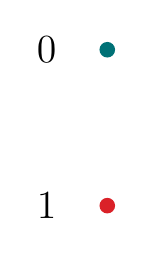
\begin{tikzpicture}[scale=0.55]
						
						\node at (0,1.8) {\Large \(0\)};
						\fill[umbcaokteal] (1.4,1.8) circle (0.18);
						
						\node at (0,-1.8) {\Large \(1\)};
						\fill[umbcred] (1.4,-1.8) circle (0.18);
						
					\end{tikzpicture}
					
					\vspace{0.4cm}
					
					{\scriptsize Classical bit stores either \(0\) or \(1\)}
					
				\end{minipage}
				
			\end{column}
			
			% -------------------------------------------------
			% Bloch sphere
			% -------------------------------------------------
			
			\begin{column}{0.33\textwidth}
				\centering
				
				\begin{minipage}[c][5cm][c]{\linewidth}
					\centering
					
					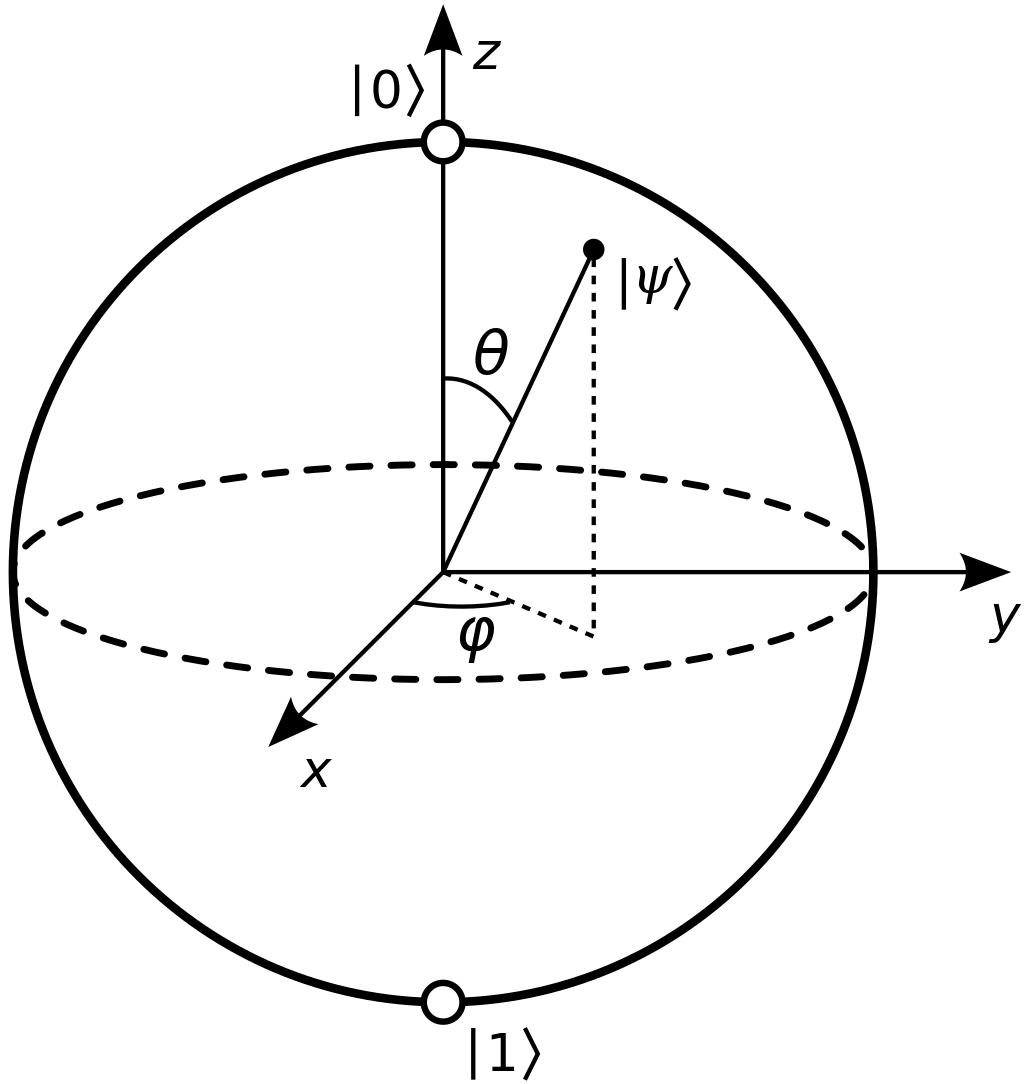
\includegraphics[width=0.78\linewidth]{bloch.png}
					
					{\scriptsize Bloch sphere of a qubit}
					
				\end{minipage}
				
			\end{column}
			
		\end{columns}
		
		A qubit may exist in a superposition:
		\[
		|\psi\rangle = \alpha |0\rangle + \beta |1\rangle,
		\qquad
		|\alpha|^2 + |\beta|^2 = 1.
		\]
		
	}
\end{frame}

% ---------------------------------------------------------
% Slide 3
% ---------------------------------------------------------

\begin{frame}{Measurement Problem}
	\Wider[2em]{
		
		A quantum state may contain multiple possible outcomes simultaneously until measured, collapsing the state probabilistically:
		\[
		|0\rangle \text{ with probability } |\alpha|^2,
		\qquad
		|1\rangle \text{ with probability } |\beta|^2.
		\]
		
		\begin{center}
			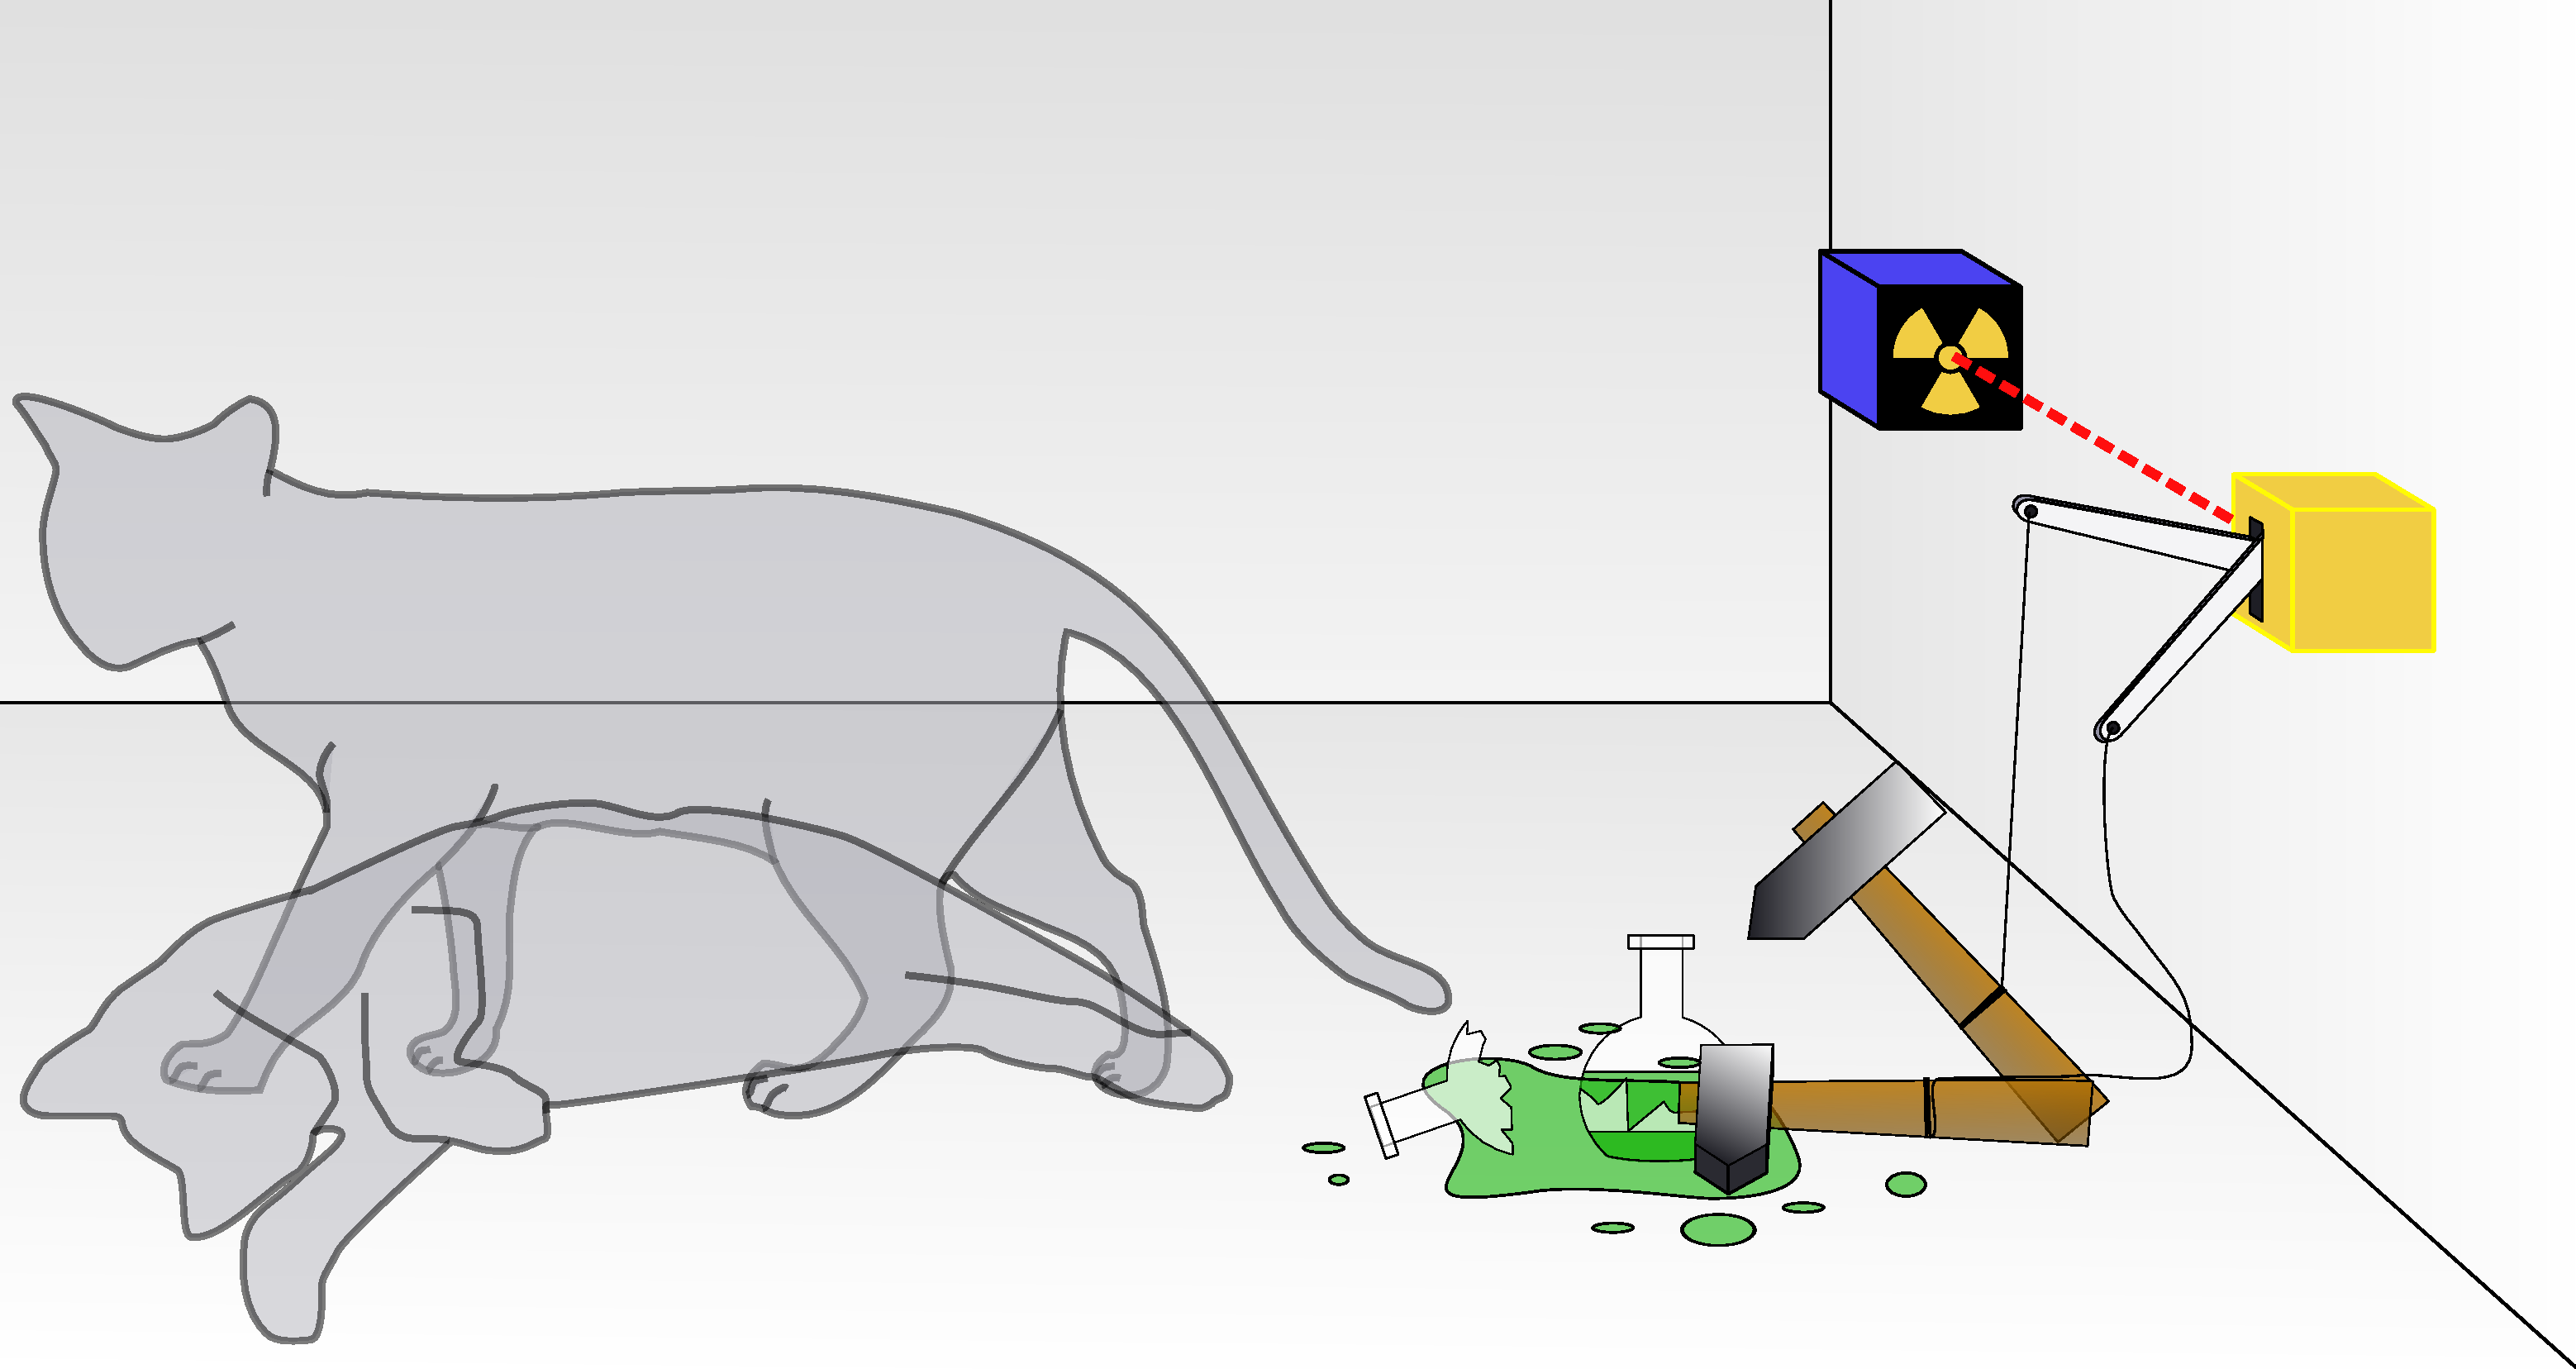
\includegraphics[width=0.32\textwidth]{Schrodingers_cat.pdf}
			
			{\scriptsize Schrödinger's cat: superposition before observation}
		\end{center}
		
		\begin{block}{Interpretation}
			Quantum systems evolve continuously until measurement.
		\end{block}
		
	}
\end{frame}

% ---------------------------------------------------------
% Slide 4
% ---------------------------------------------------------

\begin{frame}{Entanglement}
	\Wider[2em]{
		
		Two quantum systems are \textbf{entangled} when their joint state cannot be separated into independent components:
		\[
		|\psi\rangle \neq |\psi_A\rangle \otimes |\psi_B\rangle.
		\]
		
		This means:
		\begin{itemize}
			\setlength{\itemsep}{0.35em}
			\item measuring one system reveals information about the other,
			\item correlations exist beyond classical independence,
			\item strategies may become correlated through entanglement.
		\end{itemize}
		
		\begin{block}{Connection to Quantum Game Theory}
			Entanglement changes the strategic correlation structure of a game and may alter equilibrium behavior.
		\end{block}
		
	}
\end{frame}
		
		\section{Quantum Game Theory}
		
		\begin{frame}{From Classical to Quantum}
			\Wider[2em]{
				Classically, a player chooses:
				\[
				C \quad \text{or} \quad D.
				\]
				
				In the quantum version, the basis states represent classical actions:
				\[
				|C\rangle = \text{cooperate}, \qquad |D\rangle = \text{defect}.
				\]
				
				A general quantum state may be a superposition:
				\[
				|\psi\rangle = \alpha |C\rangle + \beta |D\rangle,
				\qquad |\alpha|^2 + |\beta|^2 = 1.
				\]
				
				Players do not directly choose outcomes. They apply unitary operations to qubits, and outcomes appear only after measurement.
			}
		\end{frame}
		
		\begin{frame}{EWL Quantum prisoner's dilemma}
			\Wider[2em]{
				Eisert, Wilkens, and Lewenstein proposed the following protocol:
				
				\begin{enumerate}
					\item Start with the classical state:
					\[
					|CC\rangle.
					\]
					\item Apply an entangling operator \(J\).
					\item Each player applies a local unitary strategy:
					\[
					U_A \otimes U_B.
					\]
					\item Undo the entanglement with \(J^\dagger\), then measure.
				\end{enumerate}
				
				The final state is:
				\[
				|\psi_f\rangle
				=
				J^\dagger (U_A \otimes U_B)J|CC\rangle.
				\]
			}
		\end{frame}
		
		\begin{frame}{Entanglement Parameter}
			\Wider[2em]{
				The entangling operator is commonly written as:
				\[
				J(\gamma)
				=
				\exp\left(-i\frac{\gamma}{2}D\otimes D\right),
				\qquad
				\gamma \in \left[0,\frac{\pi}{2}\right].
				\]
				
				\[
				\gamma = 0
				\quad \Rightarrow \quad
				\text{classical game}.
				\]
				
				\[
				\gamma = \frac{\pi}{2}
				\quad \Rightarrow \quad
				\text{maximally entangled quantum game}.
				\]
				
				\begin{block}{Interpretation}
					The parameter \(\gamma\) controls the transition from independent classical choices to correlated quantum strategic behavior.
				\end{block}
			}
		\end{frame}
		
		\begin{frame}{Entanglement and Equilibrium Transition}
			\Wider[2em]{
				
				\begin{center}
					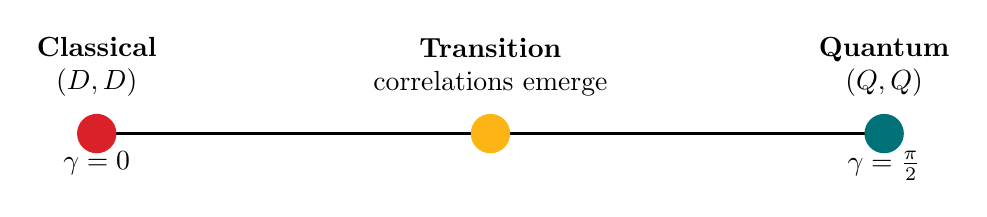
\begin{tikzpicture}[scale=1]
						
						\draw[thick,->] (0,0) -- (10,0);
						
						\fill[umbcred] (0,0) circle (0.25);
						\fill[umbcgold] (5,0) circle (0.25);
						\fill[umbcaokteal] (10,0) circle (0.25);
						
						\node[below] at (0,-0.1) {$\gamma = 0$};
						\node[below] at (10,-0.1) {$\gamma = \frac{\pi}{2}$};
						
						\node[above,align=center] at (0,0.35)
						{\textbf{Classical}\\ $(D,D)$};
						
						\node[above,align=center] at (5,0.35)
						{\textbf{Transition}\\ correlations emerge};
						
						\node[above,align=center] at (10,0.35)
						{\textbf{Quantum}\\ $(Q,Q)$};
						
					\end{tikzpicture}
				\end{center}
				
				\vspace{0.3cm}
				
				\begin{block}{Interpretation}
					Increasing entanglement changes the strategic correlation structure of the game, shifting equilibrium behavior from classical defection toward cooperative quantum equilibria.
				\end{block}
				
			}
		\end{frame}
		
		\begin{frame}{Quantum Strategies}
			\Wider[2em]{
				Players choose unitary transformations of the form:
				\[
				U(\theta,\phi)
				=
				\begin{pmatrix}
					e^{i\phi}\cos(\theta/2) & \sin(\theta/2) \\
					-\sin(\theta/2) & e^{-i\phi}\cos(\theta/2)
				\end{pmatrix}.
				\]
				
				Classical cooperation and defection are special cases:
				\[
				C = I,
				\qquad
				D =
				\begin{pmatrix}
					0 & 1 \\
					-1 & 0
				\end{pmatrix}.
				\]
				
				EWL also identifies a quantum strategy:
				\[
				Q =
				\begin{pmatrix}
					i & 0 \\
					0 & -i
				\end{pmatrix}.
				\]
			}
		\end{frame}
		
		\begin{frame}{Joint Quantum Strategy Space}
			\Wider[2em]{
				
				Players act on qubits in the joint Hilbert space:
				
				\[
				\{|CC\rangle, |CD\rangle, |DC\rangle, |DD\rangle\}.
				\]
				
				\begin{center}
					
					\renewcommand{\arraystretch}{1.8}
					
					\begin{tabular}{c c c}
						
						& $|C\rangle_{P_2}$ & $|D\rangle_{P_2}$ \\
						
						\cline{2-3}
						
						$|C\rangle_{P_1}$
						& \multicolumn{1}{|c|}{$|CC\rangle$}
						& \multicolumn{1}{c|}{$|CD\rangle$} \\
						
						\cline{2-3}
						
						$|D\rangle_{P_1}$
						& \multicolumn{1}{|c|}{$|DC\rangle$}
						& \multicolumn{1}{c|}{$|DD\rangle$} \\
						
						\cline{2-3}
						
					\end{tabular}
					
				\end{center}
				
				\vspace{0.3cm}
				
				Measurement collapses the final quantum state into one of these classical outcomes.
				
			}
		\end{frame}
		
		\begin{frame}{Expected Payoffs}
			\Wider[2em]{
				After measurement, the final quantum state produces probabilities for the four classical outcomes:
				\[
				P_{CC}, \qquad P_{CD}, \qquad P_{DC}, \qquad P_{DD}.
				\]
				
				Player A's expected payoff is:
				\[
				\mathbb{E}[u_A]
				=
				RP_{CC}+SP_{CD}+TP_{DC}+PP_{DD}.
				\]
				
				Player B's expected payoff is:
				\[
				\mathbb{E}[u_B]
				=
				RP_{CC}+TP_{CD}+SP_{DC}+PP_{DD}.
				\]
			}
		\end{frame}
		
		\begin{frame}{Equilibrium Search as Optimization}
			\Wider[2em]{
				For fixed opponent strategy \(U_B\), player A solves:
				\[
				U_A^*
				\in
				\argmax_{U_A \in \mathcal{S}}
				\mathbb{E}[u_A(U_A,U_B;\gamma)].
				\]
				
				A Nash equilibrium is a pair \((U_A^*,U_B^*)\) such that:
				\[
				\mathbb{E}[u_A(U_A^*,U_B^*)]
				\geq
				\mathbb{E}[u_A(U_A,U_B^*)],
				\]
				\[
				\mathbb{E}[u_B(U_A^*,U_B^*)]
				\geq
				\mathbb{E}[u_B(U_A^*,U_B)].
				\]
				
				\begin{block}{Learning-Theoretic View}
					The strategy space is continuous and matrix-valued, so equilibrium search resembles nonconvex policy optimization rather than finite action selection.
				\end{block}
			}
		\end{frame}
		
		\begin{frame}{Numerical Experiment}
			\Wider[2em]{
				To make the theory testable, the project can simulate the EWL game over a grid of strategy parameters:
				
				\vspace{0.15cm}
				
				\begin{enumerate}
					\item Sweep entanglement values $\gamma \in [0,\frac{\pi}{2}]$
					\item Grid-search player strategies $U(\theta,\phi)$
					\item Compute $|\psi_f\rangle = J^\dagger(U_A\otimes U_B)J|CC\rangle$
					\item Convert amplitudes into outcome probabilities: $P_{CC},P_{CD},P_{DC},P_{DD}$
					\item Plot expected payoffs and approximate best responses
				\end{enumerate}
				
				\begin{block}{Expected Output}
					Increasing $\gamma$ changes best-response behavior and when $(Q,Q)$ becomes stable under the restricted EWL strategy set.
				\end{block}
			}
		\end{frame}
		
		\section{Related Paper Analysis}
		
		\begin{frame}{Paper 1: Meyer, \textit{Quantum Strategies}}
			\Wider[2em]{
				\textbf{Main contribution:} Meyer showed that a player with access to quantum strategies can outperform a classical opponent in a simple strategic game.
				
				\vspace{0.2cm}
				
				\textbf{Relevance:}
				\begin{itemize}
					\item One of the earliest examples of quantum advantage in game theory.
					\item Superposition can behave differently from classical randomization.
				\end{itemize}
				
				\begin{block}{Relevance}
					Meyer's paper motivates the idea that strategy spaces can be expanded by quantum mechanics, and introduces the broader question: \textbf{what happens when all players have quantum strategies?}
				\end{block}
			}
		\end{frame}
		
		\begin{frame}{Paper 2: Eisert--Wilkens--Lewenstein}
			\Wider[2em]{
				\textbf{Main contribution:} EWL introduced a quantum version of prisoner's dilemma. Under \textit{maximal} entanglement, the classical equilibrium $(D,D)$ can be replaced by the quantum equilibrium $(Q,Q)$.
				
				At \((Q,Q)\), both players receive the cooperative payoff
				\[
				(R,R).
				\]
				
				\begin{block}{Interpretation}
					Entanglement allows stable cooperation \textit{without} communication.
				\end{block}
			}
		\end{frame}
		
		\begin{frame}{Paper 3: Benjamin--Hayden Critique}
			\Wider[2em]{
				\textbf{Main contribution:} Benjamin and Hayden argued that the EWL result depends strongly on the restricted set of allowed strategies. If players are allowed to use a larger set of unitary operations, then:
				\begin{itemize}
					\item the proposed quantum equilibrium may no longer be stable,
					\item counter-strategies may exist,
					\item the cooperative resolution becomes less automatic.
				\end{itemize}
				
				\begin{block}{Relevance}
					This critique turns the project from ``quantum games solve prisoner's dilemma'' into a more careful question about assumptions, strategy spaces, and equilibrium stability.
				\end{block}
			}
		\end{frame}
		
		\section{Research Direction}
		
		\begin{frame}{Learning Dynamics}
			\Wider[2em]{
				
				\vspace{1em}
				
				Parameterize each player's strategy by \((\theta,\phi)\) and update parameters using payoff feedback:
				
				\[
				(\theta_A,\phi_A)
				\leftarrow
				(\theta_A,\phi_A)
				+
				\eta \nabla_{(\theta_A,\phi_A)}
				\mathbb{E}[u_A].
				\]
				
				\[
				(\theta_B,\phi_B)
				\leftarrow
				(\theta_B,\phi_B)
				+
				\eta \nabla_{(\theta_B,\phi_B)}
				\mathbb{E}[u_B].
				\]
				
				\begin{block}{Connection to Statistical Learning}
					This resembles multi-agent policy-gradient learning: agents iteratively update parameterized strategies using observed payoff signals.
				\end{block}
				
				\begin{block}{Deliverables}
					\textbf{Worst-case:} rigorous theoretical comparison and literature review.\par
					\textbf{Best-case:} payoffs and learning trajectories from equilibrium search.
				\end{block}
			}
		\end{frame}
		
		\section{Learning Theory}
		
		\begin{frame}{Statistical Learning}
			\Wider[2em]{
				
				A player searching for a good quantum strategy is solving an optimization problem:
				\[
				\argmax_{U_A} \; \mathbb{E}[u_A(U_A,U_B)].
				\]
				
				In repeated play, agents could update strategies similar to:
				\begin{itemize}
					\item reinforcement learning,
					\item policy optimization,
					\item gradient-based learning,
					\item multi-agent learning.
				\end{itemize}
				
				\begin{block}{Interpretation}
					Quantum equilibrium search can be viewed as learning over a continuous unitary strategy space.
				\end{block}
			}
		\end{frame}
		
		\begin{frame}{Classical vs. Quantum Strategies}
			\Wider[2em]{
				A classical mixed strategy randomizes over actions:
				\[
				pC + (1-p)D.
				\]
				
				A quantum strategy transforms amplitudes:
				\[
				|\psi\rangle = \alpha |C\rangle + \beta |D\rangle.
				\]
				
				The difference is that amplitudes can interfere before measurement.
				
				\vspace{0.2cm}
				
				\begin{block}{Theoretical Claim}
					Unlike classical randomization, entanglement and interference can produce correlations unavailable to independent mixed strategies.
				\end{block}
			}
		\end{frame}
		
		\section{Takeaways}
		
		\begin{frame}{Limitations}
			\Wider[2em]{
				
				\vspace{1em}
				
				\begin{itemize}
					\item \textbf{Restricted strategy spaces:} EWL's cooperative equilibrium depends on which unitary strategies are allowed.
					\item \textbf{Physical implementation:} Real quantum systems are affected by noise and decoherence.
					\item \textbf{Equilibrium stability:} Enlarging the strategy set may introduce counter-strategies.
					\item \textbf{Learning dynamics:} It is unclear whether adaptive agents would actually converge to the quantum equilibrium.
					\item \textbf{Interpretation:} Quantum advantage may depend on whether entanglement is treated as a resource provided before the game.
				\end{itemize}
				
				\begin{block}{Open Problem}
					When does quantum game theory produce new strategic behavior rather than a reformulation of correlated/mixed classical strategies?
				\end{block}
			}
		\end{frame}
		
		\begin{frame}{Conclusion}
			\Wider[2em]{
				
				The EWL protocol, the first pioneer of quantum game theory, suggests that entanglement can convert the inefficient classical equilibrium of prisoner's dilemma into a cooperative quantum equilibrium.
				
				\vspace{0.2cm}
				
				\textbf{However}, the Benjamin--Hayden critique shows that this conclusion is not unconditional. The stability of the result depends on how the quantum strategy space is defined.
				
				\begin{block}{Key Takeaway}
					Quantum game theory serves as a theoretical bridge between equilibrium analysis, optimization, and learning.
				\end{block}
			}
		\end{frame}
		
		\begin{frame}{Future Work}
			\Wider[2em]{
				\textbf{Next steps:}
				
				\begin{itemize}
					\item implement payoff-landscape plots over \((\theta,\phi,\gamma)\),
					\item visualize whether increasing \(\gamma\) changes best-response behavior,
					\item test when \((Q,Q)\) is stable under the restricted EWL strategy set.
				\end{itemize}
				
				\begin{block}{Scope}
					Although a theoretical project, my goal is connecting the theory to statistical learning via computation/practical implementation.
				\end{block}
			}
		\end{frame}
		
		\begin{frame}{References}
			\tiny
			\setlength{\parskip}{0pt}
			\setlength{\baselineskip}{5.5pt}
			
			\begin{columns}[T,totalwidth=\textwidth]
				
				\begin{column}{0.49\textwidth}
					[1] David A. Meyer. \textit{Quantum strategies}. Phys. Rev. Lett., 82(5):1052--1055, 1999.
					
					[2] Jens Eisert, Martin Wilkens, and Maciej Lewenstein. \textit{Quantum games and quantum strategies}. Phys. Rev. Lett., 83(15):3077--3080, 1999.
					
					[3] Simon C. Benjamin and Patrick M. Hayden. \textit{Comment on ``Quantum games and quantum strategies''}. Phys. Rev. Lett., 87(6), 2001.
					
					[4] John Nash. \textit{Non-cooperative games}. Annals of Mathematics, 54(2):286--295, 1951.
					
					[5] Richard S. Sutton and Andrew G. Barto. \textit{Reinforcement Learning: An Introduction}. MIT Press, 2018.
					
					[6] Michael A. Nielsen and Isaac L. Chuang. \textit{Quantum Computation and Quantum Information}. Cambridge University Press, 2010.
				\end{column}
				
				\begin{column}{0.49\textwidth}
					[7] Lucian Busoniu, Robert Babuska, and Bart De Schutter. \textit{A comprehensive survey of multiagent reinforcement learning}. IEEE Trans. Syst., Man, Cybern. C, 38(2):156--172, 2008.
					
					[8] Richard Jankowski. \textit{Punishment in iterated chicken and prisoner's dilemma games}. Rationality and Society, 2(4):449--470, 1990.
					
					[9] Sau-Him Paul Lau and Vai-Lam Mui. \textit{Using turn taking to achieve intertemporal cooperation and symmetry in infinitely repeated \(2\times2\) games}. Theory and Decision, 72(2):167--188, 2012.
					
					[10] Kazuki Ikeda and Shoto Aoki. \textit{Infinitely repeated quantum games and strategic efficiency}. Quantum Information Processing, 20(12), 2021.
					
					[11] Thomas S. Ferguson. \textit{A Course in Game Theory}. World Scientific, 2020.
				\end{column}
				
			\end{columns}
		\end{frame}
		
		\begin{frame}
			\centering
			
			\vfill
			
			{\Huge \textcolor{umbcgold}{\textbf{Thank You!}}}
			
			\vfill
		\end{frame}
	
\end{document}